\documentclass[12pt]{article}

\usepackage[utf8]{inputenc}
\usepackage[russian]{babel}

\usepackage{amssymb}
\usepackage{amsmath}
\usepackage{amscd}
\usepackage{amsthm}
\usepackage{xcolor}

\usepackage{indentfirst}

%\usepackage{marginnote} % this is used for notes on the right margin --- \marginnote{\footnotesize txt}

\usepackage{mathtools} % for mathclap command

%\usepackage[normalem]{ulem} % for crossing text out - \sout

% Redefining \def is impossible. I tried, but it is impossible.
%\let\def_prev\def

%%%%%%%%%%%%%%%%%%%%%%%%%%%%%%%%%%%%%%%%%%%%%%%
%           MATH OPERATORS SPACING            %
%%%%%%%%%%%%%%%%%%%%%%%%%%%%%%%%%%%%%%%%%%%%%%%

\let\existstemp\exists
\let\foralltemp\forall
\renewcommand{\exists}{\: \existstemp \:}
\newcommand{\existsonly}{\: \existstemp ! \:}
\renewcommand{\forall}{\: \foralltemp \:}

%%%%%%%%%%%%%%%%%%%%%%%%%%%%%%%%%%%%%%%%%%%%%%%
%            COMMAND SHORTHANDS               %
%%%%%%%%%%%%%%%%%%%%%%%%%%%%%%%%%%%%%%%%%%%%%%%

\newcommand{\example}{{\itshape Пример. }}
\newcommand{\equals}{\Leftrightarrow}
\newcommand{\exc}{{\bfseries Упражнение. }}
\newcommand{\norm}[1]{\left\| #1 \right\|}
\newcommand{\scal}[2]{\left\langle #1, #2 \right\rangle}
\newcommand{\angular}[1]{\langle #1 \rangle}

\newcommand{\Sum}[2]{\underset{#1}{\overset{#2}{\sum}}}
\newcommand{\Int}[2]{\underset{#1}{\overset{#2}{\int}}}
\newcommand{\Ker}{\text{Ker}}

% Physicists' variant of dot product
\newcommand{\pscal}[2]{\, \langle #1 | #2 \rangle \,}
\newcommand{\bra}[1]{\, \langle #1 |}
\newcommand{\ket}[1]{| #1 \rangle \,}

\renewcommand{\leq}{\leqslant}
\renewcommand{\geq}{\geqslant}

%%%%%%%%%%%%%%%%%%%%%%%%%%%%%%%%%%%%%%%%%%%%%%%
%         THEOREM DEFINITION LINES            %
%%%%%%%%%%%%%%%%%%%%%%%%%%%%%%%%%%%%%%%%%%%%%%%

\newtheorem{lem}{Лемма}[section]
\newtheorem{note}{Замечание}[section]
\newtheorem{defi}{Определение}[section]
\newtheorem{theorem}{Теорема}[section]
\newtheorem{state}{Утверждение}[section] % statement

%%%%%%%%%%%%%%%%%%%%%%%%%%%%%%%%%%%%%%%%%%%%%%%
%             GRAPHICS INCLUSION              %
%%%%%%%%%%%%%%%%%%%%%%%%%%%%%%%%%%%%%%%%%%%%%%%

\usepackage{graphicx}

\graphicspath{{./Graphics/}}

%%%%%%%%%%%%%%%%%%%%%%%%%%%%%%%%%%%%%%%%%%%%%%%
%               DRAFT TEMPLATES               %
%%%%%%%%%%%%%%%%%%%%%%%%%%%%%%%%%%%%%%%%%%%%%%%

%\usepackage{marginnotes}
\newcommand{\todo}[1]{\marginpar{\color{red} \tiny #1}}

\begin{document}

\section{Вариационное исчисление}

	\subsection{Примеры задач вариационного исчисления}

	Прежде чем приступать к описанию методов вариационного исчисления, приведём несколько классических
	задачек, некоторые из которых мы в последствии решим.

		\subsubsection{Задача о брахистохроне}

			Рассмотрим следующую задачу: в плоскости $Oxy$ заданы две точки, требуется найти гладкую кривую, 
			по которой груз под действием силы тяжести спустится без трения за минимальное время. Эта кривая
			называется \textbf{кривой наименьшего спуска} (или \textbf{брахистохроной}).

			\todo{Картинка}

			Применим к системе закон сохранения энергии:

			\begin{align*}
				&mgy = \frac{mv^2}{2} \\
				&\begin{CD}
					v @.=@. \sqrt{2gy} @.\\
					\vspace{-27pt}\\
					\parallel @. @. @. \\
					\vspace{-27pt}\\
					\frac{dS}{dt} @. @. @.
				\end{CD}
			\end{align*}

			Где $S$ --- пройденный путь. Так как в рассматриваемой задаче искомой критерием является время,
			запишем $$\frac{dt}{dS} = \frac{1}{\sqrt{2gy}}$$

			Элемент длина дуги, описываемой функцией $y(x)$, вычисляется как:

			$$dS = \sqrt{1 + y'^2} dx$$

			То есть $\frac{dS}{dx} = \sqrt{1 + y'^2}$, откуда следует, что:
			$$\frac{dt}{dx} = \frac{dt}{dS} \frac{dS}{dx} \qquad\Rightarrow\qquad 
				T[y] = \int_0^{x_1} \frac{\sqrt{1+y'^2}}{\sqrt{2gy}} \, dx$$

			Задача поиска кривой наименьшего спуска свелась к \textit{задаче поиска минимума функционала
			$T[y]$}. Функция $y(x)$, минимизирующая $T[y]$, и будет описывать искомую кривую.

		\subsubsection{Задача о поверхность вращения минимальной площади}

			Из курса математического анализа вы знаете формулу для площади поверхности вращения, образованной
			кривой $y(x)$ на промежутке $[x_1, x_2]$:

				$$S[y] = 2 \pi \int_{x_1}^{x^2} y \sqrt{1+y'(x)^2} dx$$

			Это тоже функционал, у которого можно найти минимум. Это же в свою очередь означает, что можно
			найти поверхность наименьшей площади между двумя плоскостями: $x=x_1$ и $x=x_2$.

		\subsubsection{Изопериметрическая задача}

			\todo{Картинка}
	
			\todo{Бред же написан}

			Среди всех кривых, соединяющих две фиксированных точки, найти такую, которая имеет наименьшую
			площадь. Опять же, получится
	
			$$I[y] = \int_{x_0}^{x_1} y\sqrt{1 + y'^2}\,dx \qquad \left\{
			\begin{aligned}
				y(x_0) = y_0 \\
				y(x_1) = y_1
			\end{aligned}
			\right.$$
	
	\subsection{Простейшая задача вариационного исчисления}
	
		Рассмотрим функционал
 
		$$I[y] = \int_{x_0}^{x_1} F(x,y,y') \,dx \qquad \left\{
		\begin{aligned}
			y(x_0) = y_0 \\
			y(x_1) = y_1
		\end{aligned}
		\right. ~ ,$$
	
		где $F\in C^2$ (дважды гладкая).

		\begin{defi}
			Функция $y(x)$ называется \textbf{допустимой}, если $y$ удовлетворяет граничным условиям и
			$\forall x\, (x, y, y')\in D(F)$ .
		\end{defi}

		\todo{Есть ли способ поиска решения в $C^1$?}

		Стоит заметить, что по изначальной постановке задачи, $y \in C^1$, но предполагаемый способ решения
		даст только $y \in C^2$. Таким образом, какие-нибудь решения могут потеряться. 

		Для поиска экстремума функционала нам требуется ввести его определение. Вспомним определение экстремума функции (для определённости максимума) в точке $x=x_0$:

			$$\forall x \exists \delta: |x - x_0| < \delta \Rightarrow y(x_0) \geq y(x)$$

		Мы можем ввести определение по аналогии, но стоит вопрос в том, какую норму для функций $y(x)$ выбрать (в случае экстремума функции берётся <<норма>> от $x$ --- а это попросту модуль). Выбор стоит между $C$-нормой и $C^1$-нормой.

		В случае выбора $C$-нормы такой экстремум называется \textbf{строгим}. При выборе же $C^1$-нормы экстремум называется \textbf{слабым}. Мы рассматриваем функционалы на гладких функциях $y(x)$, поэтому дальнейшие рассуждения будут вестись только для слабых экстремумов, поскольку это проще и удобнее.

		В таком случае определение для экстремумов принимает вид:

		\begin{defi}
			$y_0(x)$ называется локальным максимумом функционала $I[y]$, если:
			$$\forall y \exists \delta: \norm{y - y_0}_{C^1} < \delta \Rightarrow I[y_0] \geq I[y]]$$
		\end{defi}

		\begin{defi}
			$y_0(x)$ называется локальным минимумом функционала $I[y]$, если:
			$$\forall y \exists \delta: \norm{y - y_0}_{C^1} < \delta \Rightarrow I[y_0] \leq I[y]]$$
		\end{defi}

		\lecture{12}
	
		\subsubsection{Уравнение Эйлера}
	
			Как было замечено ранее, нашей задачей будет поиск локальных экстремумов этого функционала. В 
			курсе математического анализа необходимым условием локального экстремума было равенство нулю
			частных производных или, другими словами, равенство нулю производной по всем касательным в данной
			точке.
	
			Здесь будет использоваться похожее условие. Пусть функция $y(x)$ является экстремумом 
			рассматриваемого нами функционала $I[y]$. Вместо касательного вектора мы рассмотрим
			функцию $h(x)$, такую, что
			$$h \in C^{\infty} \qquad \supp(h) \subset (x_0, x_1)$$
	
			\todo{Почему она будет допустимой?}
			Тогда, если $y(x)$ --- допустимая функция, то при достаточно малых $\varepsilon$,
			$y(x) + \varepsilon h(x)$ тоже будет допустимой.
			
			Также введём функцию $J(\varepsilon) = I(y + \varepsilon h(x))$:

			$$J(\varepsilon) = \int_{x_0}^{x_1} F(x, y(x) + \varepsilon h(x), y'(x) + \varepsilon h'(x))\,dx$$

			Обозначим для функции $F$ её частные производные как $F_x, F_y, F_{y'}$. Стоит отметить, что
			частная производная берётся в предположении независимости переменной дифференцирования от
			остальных переменных функции.

			Тогда производная функции $J(\varepsilon)$ примет вид:
	
			$$J'(\varepsilon)\lims{\varepsilon = 0}{} = \int_{x_0}^{x_1} \Big( F_{y}h(x) - F_{y'}h'(x) \Big)\,dx$$
	
			Проинтегрируем второе слагаемое в подынтегральном выражении по частям. Здесь мы делаем ранее
			упомянутое отклонение от постановки задачи: потребуется, чтобы функция $F \in C^2$, а не $C^1$.

			$$\int_{x_0}^{x_1} F_{y'}h'(x) \,dx = \off{F_{y'}h(x) \lims{x_0}{x_1}} - \int_{x_0}^{x_1} h(x)(\frac{d}{dx} F_y)\,dx$$

			$$J'(\varepsilon)\lims{\varepsilon = 0}{} = \int_{x_0}^{x_1}h(x)\cdot(F_y - \frac{d}{dx}F_{y'}) \,dx$$

			\todo{Почему бы не просто лемму Лагранжа?}

			Из теории обобщённых функций известно, что, если регулярная обобщённая функция $f$ порождена
			непрерывной и $\forall h\:\scal{F}{h}~=~0$, то $f = 0$. Таким образом, из условия $J' = 0$
			получаем \textbf{уравнение Эйлера}:

			\begin{equation} \label{eq:Euler}
				F_y - \frac{d}{dx}F_{y'} = 0 
			\end{equation}
	
			Равенство нулю уравнения (\ref{eq:Euler}) в точности совпадает с условием равенства нулю
			производной по всем касательным векторам.
	
			\begin{defi}
				Функция $f(x) \in C^2$, которая является решением уравнения уравнения Эйлера, называется
				\textbf{экстремалью}.
				функционала $I[y]$.
			\end{defi}
			
			\opt{
				Обратите внимание, что уравнение Эйлера --- это лишь необходимое условие локального
				экстремума функционала $I[y]$. Экстремали являются функциями подозрительными на экстремум, но
				могут не являться экстремума. Для дальнейшего изучения требуются достаточные условия, что
				находится за рамками нашего курса.
			}

			Рассмотрим три ситуации, когда уравнение (\ref{eq:Euler}) допускает понижение порядка:

			\begin{enumerate}
				\item $F(x,y,y') = F(x,y)  \Rightarrow \mathbf{F_y = 0}$
				\item $F(x,y,y') = F(x,y') \Rightarrow \mathbf{F_{y'} = C}$
				\item $F(x,y,y') = F(y,y') \Rightarrow \mathbf{y'F_{y'} - F = C}$

					Такое уравнение возникает в задаче нахождения минимальной поверхности вращения. Здесь
					понижение порядка не столь тривиально.

					Рассмотрим функцию $(y'F_{y'} - F)$. Продифференцируем её по $x$:
					$$\frac{d}{dx}(y'F_{y'} - F) =
			  			\off{y''F_{y'}} + y'(\frac{d}{dx}F_{y'}) - F_yy' - \off{F_{y'}y''} = 
			  			y'(\frac{d}{dx}F_{y'} - F_y)$$

					В скобках стоит уравнение Эйлера. Тогда, если $y$ --- экстремаль, то это выражение равно
					нулю и уравнение получается более простое:

					$$\mathbf{y'F_{y'} - F = C}$$
			\end{enumerate}

	\subsection{Решение задачи о брахистохроне}

		Теперь у нас есть вся необходимая теория для решения задачи о брахистохроне --- кривой наискорейшего
		спуска.

		$$I[y] = \int_0^{x_1} \frac{\sqrt{1+y'^2}}{\sqrt{y}} \,dx$$

		Как видим, в данной задаче $F$ не зависит явно от $x$. Значит, выполняется случай (3).

		$$y'\frac{y'}{\sqrt{y(1+y'^2)}} - \frac{\sqrt{1+y'^2}}{\sqrt{y}} = C$$
		$$\frac{1}{\sqrt{y(1+y'^2)}} = C$$
		$$y(1+y'^2) = C_1$$

		Здесь и далее наиболее частым приёмом для решения дифференциальных уравнений является введение параметра:

		$$y' = ctg(v)$$
		$$y = C_1 \sin^2(v) = \frac{C_1}{2}(1 - \cos(2v))$$

		Осталось найти $x = x(v)$, и решение будет получено.

		$$\frac{dx}{dv} = \frac{dy}{dv} \frac{1}{y'} = 
			\frac{C_1\sin(2v)}{ctg(v)} = \frac{2C_1 \sin^2(v)\cos(v)}{\cos(v)} = C_1\big(1 - cos(2v)\big)$$

		Интегрируя данное уравнение по $v$, получаем $x(v)$:

		$$x(v) = C_1\left(v - \frac{\sin(2v)}{2}\right) + C_2$$
	
		Получаем параметризованное решение уравнения:

		\begin{align*}
				x = \frac{C_1}{2} \big(t - \sin(t)\big) + C_2 \\
				y = \frac{C_1}{2} \big(1 - \cos(t)\big)
		\end{align*}
	
		Из начальных условий $x(t=0) = 0$, откуда следует, что $C_2 = 0$.

		Получаем окончательный ответ на задачу о брахистохроне:

		\todo{Другая картинка}

		\begin{figure}[H]
			\begin{subfigure}[c]{0.5\textwidth}
			\begin{align*}
					x = C \big(t - \sin(t)\big) \\
					y = C \big(1 - \cos(t)\big)
			\end{align*}		
			\end{subfigure}
			~
			\begin{subfigure}[c]{0.5\textwidth}
					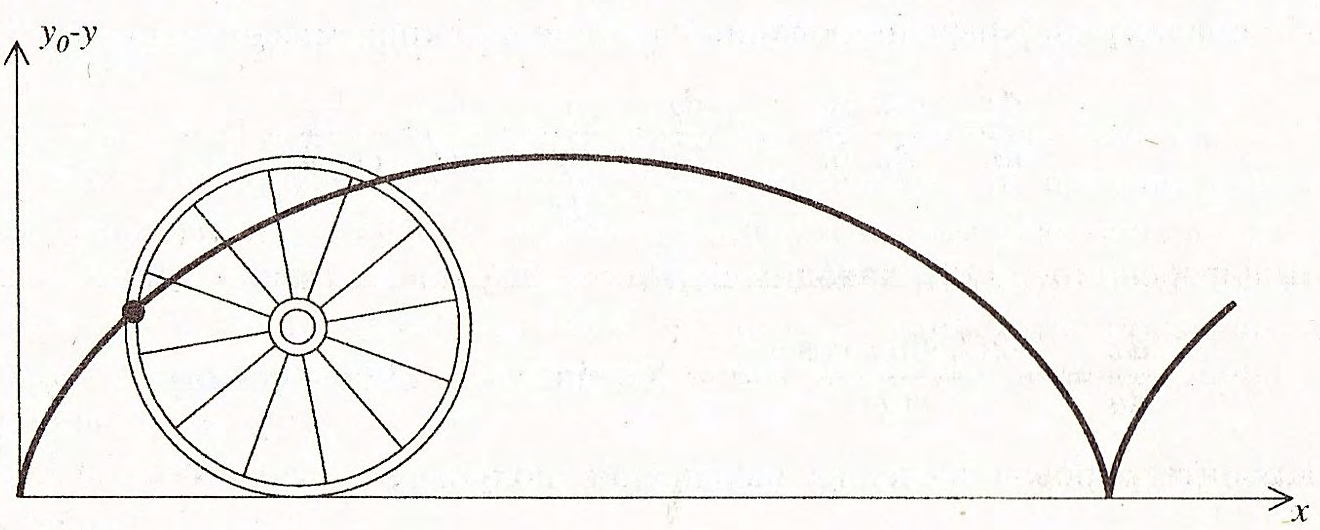
\includegraphics[width=0.8\textwidth]{../Graphics/Lectures-12-cycloid.png}
					\caption{\footnotesize Циклоида \copyvar{С. 22.}}
			\end{subfigure}
		\end{figure}
	
		Видим, что кривой наименьшего спуска является циклоида.

	\subsection{Более сложные задачи}

		Для решения некоторых задач вариационного исчисления может потребоваться большее число функций или
		независимых переменных. К примеру, задача нахождения геодезической кривой, в которой требуется найти
		$x(t), y(t), z(t)$, которые определяют кратчайший путь между двумя точками на поверхности трёхмерной
		фигуры.

		Рассмотрим подобные случаи.

		\subsubsection{Задача с несколькими функциями}

			Итак, если есть несколько функций $y$:
			$$F = F(x, y_1, y_1', y_2, y_2',\ldots)$$

			Тогда просто записывается система уравнений Эйлера:
			$$\left\{
			\begin{aligned}
				F_{y_1} - \frac{d}{dx}F_{y_1'} = 0 \\
				\dots\\
				F_{y_n} - \frac{d}{dx}F_{y_n'} = 0
			\end{aligned}
			\right.$$

		\subsubsection{Задача с производными высоких порядков}

			Рассмотрим случай, когда появляются производные более высоких порядков. 
			$$F = F(x, y, y', \ldots, y^{(k)})$$
			
			Как и раньше, введём функцию $J(\varepsilon) = I[y + \varepsilon h]$. $J'(\varepsilon)$. Её
			производная запишется следующим образом:

			$$J'(\varepsilon)\lims{\varepsilon = 0}{} = \int_{x_0}^{x_1} (F_y h(x) + F_{y'}h'(x) 
			+ F_{y''}h''(x) + \ldots + F_{y^{(k)}}h^{(k)})\,dx$$

			Первое слагаемое ранее уже интегрировали по частям: 
			$$\int_{x_0}^{x_1} F_{y'}h'(x)\,dx~=~-~\int_{x_0}^{x_1} h(x)\left(\frac{d}{dx} F_{y'}\right)\,dx$$

			Рассмотрим таким же образом следующее слагаемое:

			$$\int_{x_0}^{x_1} F_{y''}h'' \,dx = \off{h'(x)F_{y''}\lims{x_0}{x_1}} - \int_{x_0}^{x_1} h'(x)\frac{d}{dx}F_{y''} \,dx
	  		= \off{-h(x)\frac{d}{dx} F_{y''}\lims{x_0}{x_1}} + \int_{x_0}^{x_1} h(x) \frac{d^2}{dx^2}F_{y''} \,dx$$

			Как и ранее, выделенные серым слагаемые равняются нулю из-за того, что функции $h^{(k)}(x)$ равны
			нулю на краях отрезка $[x_0, x_1]$.

			Преобразовав все слагаемые таким образом, перепишем $J'(\varepsilon)$:
			$$\int_{x_0}^{x_1} h(x)
				\underbrace{\left(F_y - \frac{d}{dx}F_{y'} + \frac{d^2}{dx^2}F_{y''} - 
				\ldots + (-1)^k\frac{d^k}{dx^k}F_{y^{(k)}}\right)}_{f(x, y, \ldots, y^{(k)})} \,dx$$

			Так же как и раньше, необходимым условием будет являться выполнение уравнения $f = 0$.
	
			\begin{equation} \label{eq:EulerPoisson}
				F_y - \frac{d}{dx}F_{y'} + \frac{d^2}{dx^2}F_{y''} - 
				\ldots + (-1)^k\frac{d^k}{dx^k}F_{y^{(k)}} = 0
			\end{equation}
	
			Уравнение (\ref{eq:EulerPoisson}) называется \textbf{уравнением Эйлера-Пуассона}.

		\subsubsection{Задача с несколькими независимыми переменными}

			Осталось рассмотреть ситуацию, когда возникает несколько независимых переменных. Тогда рассмотрим
			функцию $z = z(x,y)$ и функционал:

			$$I[z] = \underset{D\hspace{10pt}}{\iint} F(x, y, z, z'_x, z'_y) \,dxdy$$
	
			Здесь мы снова введём $h \in C^{\infty}$, $\supp(h) \subset D$, где $D$ --- открытая область.
			Также введём $J(\varepsilon) = I[z + \varepsilon h]$ и снова запишем её производную:

			$$J'(\varepsilon)\lims{\varepsilon = 0}{} = 
	  		\underset{D\hspace{10pt}}{\iint} (F_zh + \underline{F_{z'_x}h'_x} + \underline{F_{z'_y}h'_y}) \,dxdy$$

			Чтобы получить уравнение на экстремали, нужно получить $h(x)$ вместо её производных в
			подчёркнутых слагаемых.
	
			\begin{align*}
				\frac{d}{dx}(h F_{z'_x}) = \underline{h'_xF_{z'_x}} + h\frac{d}{dx}F_{z'_x} \\
				\frac{d}{dy}(h F_{z'_y}) = \underline{h'_yF_{z'_y}} + h\frac{d}{dy}F_{z'_y}
			\end{align*}

			Перепишем $J(\varepsilon)$, выразив подчёркнутые слагаемые:
	
			$$
				J'(\varepsilon)\lims{\varepsilon = 0}{} = 
				\underset{D\hspace{10pt}}{\iint} \left( h\cdot\left(F_z - \frac{d}{dy}F_{z'_y} - \frac{d}{dx}F_{z'_x}\right) \right) \,dxdy
				+ \underset{D\hspace{10pt}}{\iint} \left(\frac{d}{dx}(hF_{z'_x}) + \frac{d}{dy}(hF_{z'_y}) \right) \,dxdy
			$$

			Второй интеграл может быть преобразован по теореме Стокса из векторного анализа. В двумерном случае (часто называемом формулой Грина):

			$\iint_{D} (P\,dx + Q\,dy) = \oint_{\partial D} (Q_x - P_y) dx dy$.

			Отсюда получаем:

			$$
				J'(\varepsilon)\lims{\varepsilon = 0}{} = 
				\underset{D\hspace{10pt}}{\iint} \left( h\cdot\left(F_z - \frac{d}{dy}F_{z'_y} - \frac{d}{dx}F_{z'_x}\right) \right) \,dxdy
				+ \underbracket{\underset{\partial D}{\oint} \left(hF_{z'_x}\,dy + hF_{z'_y}\,dx \right)}_{=0}
			$$

			Второй интеграл равняется нулю, так как функция $h(x, y)\lims{\partial D}{} \equiv 0$ потому что $\supp(h) \subset D$.

			Полученное уравнение
			$$F_z - \frac{d}{dy}F_{z'_y} - \frac{d}{dx}F_{z'_x} = 0$$
			называется \textbf{уравнением Эйлера-Остроградского}.

			\example{Интеграл Дирихле}. Рассмотрим функционал вида 
	
				$$I[z] = \iint\limits_D (z_x'^2 + z_y'^2)^2 \,dxdy$$
	
				Рассматриваемый интеграл называется интегралом Дирихле. Получим выражение для экстремалей
				функционала $I[z]$.
	
				$$\off{F_z} - \frac{d}{dy} F_{z'_y} - \frac{d}{dx} F_{z'_x} = 0$$
				$$-\frac{d}{dy} 2z'_y - \frac{d}{dx} 2z'_x = 0$$
				$$z''_{yy} + z''_{xx} = 0$$
	
				Таким образом, экстремалями этого функционала являются гармонические функции.

		\subsubsection{Задача с незакреплёнными концом. Условие трансверсальности}

			$$I[y] = \int_{x_0}^{x_1} F(x, y, y')dx \qquad y(x_0) = y_0$$
	
			\begin{figure}
				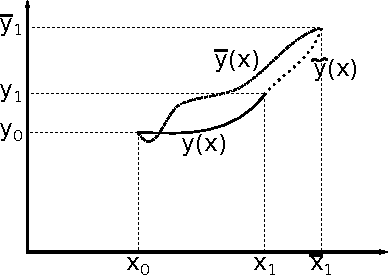
\includegraphics[width=0.8\textwidth]{./../Graphics/Lectures-12-unknowntask.pdf}
			\end{figure}
	
			Продолжим функцию $y(x)$ так, чтобы её продолжение $\tilde{y}(x) \in C^1$.
	
			Введём $\rho(y, \tilde{y}) = \norm{y - \tilde{y}} + \sqrt{(x_1 - \bar{x_1})^2 + (y_1 - \bar{y_1})^2}$. Назовём $\rho$ расстоянием между двумя этими функциями.

			Для дальнейших вычислений введём следующие обозначения:
	
			$$
				\left\{
				\begin{aligned}
					h(x) = \overline{y} - y \\
					\delta x = \overline{x_1} - x_1
					\delta y = \overline{y}(x_1) - y(x_1)
				\end{aligned}
				\right.
			$$

			$$I[\overline{y}] - I[y] = 
	  			\underbracket{\int_{x_0}^{x_1} (F(x, y + h, y' + h') - F(x, y, y')) \,dx}_{I_1} +
	  			\underbracket{\int_{\overline{x}_0}^{\overline{x}_1} F(x, \overline{y}, \overline{y}') \,dx}_{I_2}$$
	  
			В подынтегральном выражении для $I_2$ стоит непрерывная функция. Значит, можем воспользоваться
			теоремой о среднем.
	
			\opt{
				\begin{theorem*}
					Пусть функция f(x) непрерывна на $[x_1, \overline{x}_1]$, тогда 
					$\exists x_C\in[x_1,\overline{x}_1]\;\;
					\int\limits_{x_1}^{\overline{x}_1}f(x)dx = f(x_C)(\overline{x}_1 - x_1)$.
				\end{theorem*}
			}
	
			Положим некоторое значение $x_C \in [x_0, x_1]$. Тогда 
			$$I_2 = \delta x_1 F(x, \overline{y}, \overline{y}')\lims{x = x_C}{} 
			= \delta x_1 F\big(x_1, \overline{y}(x_1), \overline{y}'(x_1)\big) + o(\delta x_1)$$
	
			Приращение интеграла $I_1$ можно записать по формуле Тейлора:
			$$f(x + h) = f(x) + df(x) \angular{h} + o(\mod{h})$$
			Таким образом, 
			$$I_1 = \int_{x_0}{x_1} (F_yh - F_{y'}h') \,dx + o\big(\rho(y, \overline{y})\big)$$
	
			$o(\ldots)$ ушло из подынтегрального выражения, так как интеграл берётся по конечному промежутку,
			а умножение $o(\ldots)$ на константу ничего не меняет. Итак, интегрируем второго слагаемое по
			частям:
	
			$$I_1 = \int_{x_0}{x_1} h\cdot(F_y - \frac{d}{dx}F_{y'}) \,dx + hF_{y'}\lims{x_0}{x_1} + o(\ldots) = \int_{x_0}^{x_1} h\cdot(F_y - \frac{d}{dx}F_{y'}) \,dx + h(x_1) F_{y'}\lims{x = x_1}{}$$

			\lecture{13}

			Отсюда получаем:

			$$\Delta I = \int_{x_0}^{x_1} (F_y - \frac{d}{dx} F_{y'})h(x)\,dx + h(x_1)F_{y'}\lims{x=x_1}{} + 
	  		F\lims{x=x_1}{}\cdot \delta x_1 + o(\rho(y,\tilde{y}))$$

			Преобразуем $h(x_1)$. Как было записано ранее, $h(x_1) = \bar{y}(x_1) - y(x_1)$:

			$$\bar{y}(\bar{x}_1) - \bar{y}(x_1) = y'(x_1 + \theta \delta x_1)\cdot \delta x_1 
			= y'(x_1) \delta x_1 + o(\rho(y, \bar{y}))$$

			Тогда сможем выразить $\bar{y}$ через $y$:
			$$h(x_1) = \bar{y}(x_1) - y(x_1) = \underbracket{\bar{y}(\bar{x}_1) - y(x_1)}_{\delta y_1}
	  		- y'(x_1)\delta x_1 + o(\rho(y, \bar{y}))$$

			\begin{align*}
				\Delta I = \int_{x_0}^{x_1} \left(F_y - \frac{d}{dx}F_{y'}\right)h(x)\,dx
				+ \delta x_1\cdot(F - y'F_{y'}) \lims{x=x_1}{}
				+ \delta y_1 \cdot F_{y'}\lims{x=x_1}{}
			\end{align*}

			В вариационном исчислении величина $\Delta I$ зачастую называется вариацией функционала (по
			аналогии с дифференциалом функции). Необходимым условием экстремума будет $\Delta I = 0$. Таким
			образом, приходим к следующим уравнениям:

			\begin{equation}
				\label{eq:preTraversal}
				\begin{cases}
				&F_y - \frac{d}{dx} F_{y'} = 0 \\
				&(F - y'F_{y'})\lims{x = x_1}{} \delta x_1 + F_{y'} \lims{x=x_1}{}\delta y_1 = 0
				\end{cases} 
			\end{equation}

			\off{(Без доказательства)} Если решать задачу где и левый конец функции тоже не закреплён, то
			$\Delta I$ запишется как:
			\begin{align*}
				\Delta I = \int_{x_0}^{x_1} (F_y - \frac{d}{dx}F_{y'})h(x)\,dx~+~ 
				\delta x\cdot(F - y'F_{y'})\lims{x = x_0}{x = x_1}~+~ \\
				~+~\delta y_1 \cdot F_{y'} \lims{x=x_1}{}-~\delta y_0 \cdot F_{y'} \lims{x=x_0}{}
			\end{align*}

			\opt{\off{Популярными граничными условиями являются $F_{y'}\lims{x=x_0}{}=F_{y'}\lims{x=x_1}{}=0$}}

			\todo{Картинка}
			Если задать, что правый конец экстремали лежит на некоторой функции $\psi(x)$:
			$$\delta y_1 = \psi'(x_1) \delta x_1 + o(\delta x_1)$$

			Тогда условие (\ref{eq:preTraversal}) перепишется как:
			$$
				\begin{cases}
					&F_y - \frac{d}{dx} F_{y'} = 0 \\
					&\delta x_1 \cdot (F - y'F_{y'} + \psi' F_{y'})\lims{x=x_1}{} + o(\delta x_1) = 0
				\end{cases} 
			$$

			Уравнение
			\begin{equation}
				\label{eq:traversal}
				(F - y' F_{y'} + \psi' F_{y'})\lims{x=x_1}{} = 0
			\end{equation}
			называется \textbf{условием трансверсальности}.

			Рассмотрим частный случай, когда функция $F$ имеет вид $F(x, y, y') = f(x,y) \sqrt{1+y'^2}$.
			Подставляя $F$ в \ref{eq:traversal}, получаем:

			$$
				\left( f \sqrt{1+y'^2} - y' f \frac{y'}{\sqrt{1+y'^2}} + \psi' f \frac{y'}{\sqrt{1+y'^2}} \right) \lims{x=x_1}{}
			$$

			После простых преобразований получаем упрощённое условие трансверсальности:

			$$\left( \psi' y' \right) \lims{x=x_1}{} = -1$$

			Производные от функций можно трактовать как коэффициент наклона касательной в точке $x=x_1$, а равенство их произведения $-1$ означает перпендикулярность этих касательных. Таким образом, в случае, если $F(x, y, y') = f(x,y) \sqrt{1+y'^2}$, то оптимальным путём будет тот, который придёт в точку $x=x_1$ перпендикулярно функции $\psi(x)$.

	\subsection{Решение изопериметрической задачи}

		\todo{перепроверить, местами чушь написана}

		Пусть даны функции 
		$$x(t),\qquad y(t)$$
		с заданными граничными условиями:
		$$x(t_0) = x(t_1) = x_0 \qquad y(t_0) = y(t_1) = y_0$$

		Задача --- максимизировать площадь $S[x,y] = \int_{t_0}^{t_1}x(t)y'(t) dt$ при условии, что периметр
		$l[x,y] = \int_{t_0}^{t_1} \sqrt{\dot{x}^2(t) + \dot{y}^2(t)}\,dt$ фиксирован.

		В более общей формулировке задача звучит так: найти минимум функционала
		$I[y] = \int_{x_0}^{x_1} F(x,y,y')\,dx$, если несколько функционалов того же вида постоянны
		$J_k[y] = \int_{x_0}^{x_1} G_k(x,y,y')\,dx = C_k$. (Если считать $G_k$ дельта-функцией, то граничные
		условия тоже можно записать в таком виде.)

		Для нахождения экстремума в многомерном случае в курсе математического анализа рассматривается
		равенство нулю скалярного произведения градиента на касательную к многообразию. Нужно, чтобы
		производная вдоль любого вектора, касательного к поверхности,

		\begin{equation}g_i(x) = C_i, \qquad g_1\ldots g_m \label{eq:Surface}\end{equation}

		равнялась нулю. В выбранной точке $x$ касательное пространство является ортогональным дополнением
		к $m$ градиентам из (\ref{eq:Surface}). Следовательно, обязательным образом
		
		$$\nabla f = \sum_i \lambda_i \nabla g_i \quad \Rightarrow \quad f = \sum_i \lambda_i g_i$$

		С этими утверждениями из математического анализа вы уже знакомы. Теперь рассмотрим, как они
		применяются в нашей задаче. Нужно, чтобы вариация функционалов $J_k$ равнялась нулю:
		$\delta J_k = 0$.

		На каждое $G_k$ получается уравнение
		$$\int_{x_0}^{x_1} \left(\underline{G_{k_y} - \frac{d}{dx}G_{k_{y'}}}\right) h(x)\,dx = 0$$	
		где подчёркнутое выражение играет роль градиента. Таким образом,
		$$\delta I = \int_{x_0}^{x_1} \left(F - \frac{d}{dx}F_{y'}\right)h(x) \,dx 
	  	= \int_{x_0}^{x_1} \left(\sum_i \left(\lambda_i G_{i_y} - \frac{d}{dx}G_{i_{y'}} \right)\right)h(x) 			\,dx$$
	  
		Таким образом, должно выполняться условие
		\todo{Наверное, здесь должно быть $h(x)$}
		$$\int_{x_0}^{x_1} \left(F - \sum_i \lambda_i G_i\right) \,dx = 0$$

		Ничего не мешает нам считать, что $F(\ldots) = G_0$, тогда $\lambda_0 = 1$. Так как 
		$F$ и $G_i$ --- функции одинакового вида, можно внести $F$ в граничные условия и решать
		задачу для какого-нибудь $G_i$. Эти высказывания формируют \textbf{принцип взаимности}.

		\off{Таким образом, изопериметрическая задача равносильна нахождению минимального периметра при 
		фиксированной площади.}

	\subsection{Нахождение геодезических кривых}

		\begin{defi}
			\textbf{Геодезическая кривая} --- кратчайшая кривая, соединяющая две точки на поверхности.
		\end{defi}

		Не будем приводить здесь доказательства рассматриваемого метода, просто представим его <<рецепт>>.

		В качестве примера рассмотрим задачу о нахождении геодезических кривых на поверхности сферы.
		Рассматривается функционал следующего вида:
		$$I[x] = \int_{t_0}^{t_1} F(t,x,\dot{x})\,dt \qquad x \in \mathbb{R}^n$$

		То есть существует $n$ функций, описывающих путь по искомой кривой. В исходной задаче такой
		функционал равен $F(t,x,\dot{x}) = \sqrt{\dot{x}^2 + \dot{y}^2 + \dot{z}^2}$, то есть длине
		пути.

		Потребуется ввести граничные условия, ограничивающие область поиска:
		\begin{equation} \label{eq:GeodSurface}
			g_i(t, x, \dot{x}) = 0 \qquad i = 1,\ldots k \qquad
			\begin{aligned}
				x(t_0) = x_0 \\
				x(t_1) = x_1
			\end{aligned}
		\end{equation}

		Рассмотрим ещё один функционал:

		\todo{Здесь, видимо, тоже должно быть $h(x)$}
		$$J[x] = \int_{t_0}^{t_1} \left(F(t,x,\dot{x}) + \sum_{i=1}^k \lambda_i(t) g_i(t)\right)\,dt$$

		Сделаем важное предположение: для $F(\ldots)$, экстремали функционала $I[x]$, обязятельно найдётся
		$k$ функций $\lambda_i(t)$, таких, что решение будет представляться экстремалями функционала $J[x]$.
		При этом, $\lambda_i(t)$ находятся из уравнения Эйлера и граничных условий (\ref{eq:GeodSurface}).

	\subsection{Уравнение колебаний струны}

		\todo{Добавить из семинаров поиск уравнения колебания струны!}

\end{document}
